

\documentclass[11pt]{article}
\usepackage{graphicx}
\usepackage{times}
\usepackage{amssymb}
\usepackage{float}
\usepackage{amsmath,amssymb,amsfonts,bm}

\newcount\refno\refno=1
\def\ref{\the\refno \global\advance\refno by 1}
\def\ux{\underline{x}}
\def\uw{\underline{w}}
\def\ut{\underline{\theta}}
\def\umu{\underline{\mu}}
\def\be{p_e^*}
\newcount\eqnumber\eqnumber=1
\def\eq{\the \eqnumber \global\advance\eqnumber by 1}
\def\eqs{\eq}
\def\eqn{\eqno(\eq)}

 \pagestyle{empty}
\def\baselinestretch{1.1}
\topmargin1in \headsep0.3in
\topmargin0in \oddsidemargin0in \textwidth6.5in \textheight8.5in
\begin{document}
\setlength{\parskip}{1.2ex plus0.3ex minus 0.3ex}


\thispagestyle{empty} \pagestyle{myheadings} \markright{Homework
5: CS 274A, Probabilistic Learning: Winter 2019}



\title{CS 274A Homework 5}
\author{Caleb Nelson}
\date{Due Date:  11am  Monday March 4th}

\maketitle


\section*{Instructions and Guidelines for Homeworks}
 \begin{itemize}

\item
Please answer all of the questions and submit a scanned copy of your written solutions to Gradescope 
(either hand-written or typed are fine as long as the writing is legible). 
%Code (if requested) should be submitted to the EEE dropbox. No
%need to submit any code unless we request it.

\item
All problems are worth 10 points unless otherwise stated.  All homeworks will get equal weight in computation of the final grade for the class.
 \item
The homeworks are intended to help you work through the concepts
we discuss in class in  more detail. It is important that you try
to solve the problems yourself. The homework problems are important to help you better
learn and reinforce the material from class. If you don't
do the homeworks you will likely have difficulty in the exams
later in the quarter.

\item If you can't solve a
problem, you can discuss it {\it verbally} with another student. However, please note that before you submit your homework solutions you
are not allowed to view (or show to any other student) any {\it written material} directly related to the homeworks, including other students' solutions or drafts of solutions, solutions from previous versions of this class, and so forth. The work you hand in should be your own original work.

\item You are allowed to use reference materials in your solutions, such as class notes, textbooks,  other reference material (e.g., from the Web), or solutions to other problems in the homework. It is strongly recommended that you first try to solve the problem yourself, without resorting to looking up solutions elsewhere. If you base your solution on material that we did not discuss in class, or is not in the class notes, then you need to clearly provide a reference, e.g., ``based on material in Section 2.2 in ....."


\item
In problems that ask for a proof you should submit a complete mathematical
proof (i.e., each line must follow logically from the preceding one, without
``hand-waving"). Be as clear as possible in explaining
 your notation and in stating your reasoning as you go from line to line.  


\item
If you wish to use LaTeX to write up
your solutions you may find it useful to use the .tex file for  this homework
that is posted on the Web page. 






\end{itemize} 


\subsection*{Problem \ref:  Maximum Likelihood Estimation for Least-Squares Regression}
In class we showed that least squares regression could be related to a conditional  Gaussian likelihood. Assume we have training data in the form  $D = \{ (x_i, y_i) \}$, where $x$ and $y$ are both 1-dimensional and $i=1,\ldots,N$. Say we assume a model of the form $E[y] = a x + b$, with $y$ having Gaussian noise with variance $\sigma^2$ and mean $E[y]$. Derive equations for the maximum likelihood estimates for each of $a$, $b$, and $\sigma^2$.
\begin{equation}
	p(y_i|x_i,a,b,\sigma^2) = \frac{e^{\frac{-(y_i-x_ia-b)^2}{2\sigma^2}}}{\sqrt{2\pi\sigma^2}}
\end{equation}
since $l(y|x,a,b,\sigma^2) = log(L(y|x,a,b,\sigma^2)) = log(\prod_i^N p(y_i|x_i,a,b,\sigma^2))$, 
\begin{equation}
	l(y|x,a,b,\sigma^2) = \sum_i^N log(\frac{1}{\sqrt{2\pi\sigma^2}}) + \frac{-(y_i-x_ia-b)^2}{2\sigma^2}
\end{equation}
\begin{itemize}
\item
	$\frac{\delta l}{\delta a} = \sum_i^N \frac{-2(y_i-x_ia-b)x_i}{2\sigma^2}$.
	Setting this equal to 0 and solving for $a$ give us $\sum_i^N y_i - \sum_i^N x_i a - Nb = 0$,
	$\hat{a}_{MLE} = \frac{\sum_i^N y_i - Nb}{\sum_i^N x_i}$

\item
	$\frac{\delta l}{\delta b} = \sum_i^N \frac{-2(y_i-x_ia-b)}{2\sigma^2}$. 
	Setting this equal to 0 and solving for $b$ give us $\sum_i^N y_i - \sum_i^N x_i a - Nb = 0$,
	$\hat{b}_{MLE} = \frac{1}{N}\sum_i^N (y_i - x_ia)$

\item
	$\frac{\delta l}{\delta \sigma^2} = -\frac{n}{2\sigma^2} + \sigma^{-4} \sum_i^N (y_i-x_ia-b)^2$.
	Setting this equal to 0 and solving for $\sigma^2$ gives \\
	$\hat{\sigma^2}_{MLE} = \frac{1}{n}\sum_i^N (y_i-x_ia-b)^2$
\end{itemize}

\subsection*{Problem \ref:  Convexity of Log-Loss/Logistic Objective Function} 
Consider a logistic regression model with parameters $\ut$, and with
labeled training data $D = \{ (\ux_i, y_i) \}, 1 \le i \le N$, where $y_i \in \{0,1\}$ are class labels and $\ux_i$ are
$d$-dimensional feature vectors (you can assume that the first component of $\ux_i$ is set to the constant 1).
Prove that  the log-loss objective function (i.e., the negative of the log-likelihood for a 2-class problem) is {\it convex} as a function of the parameters $\ut$. In your proof you can use the fact that a function is convex if and only if the $p \times p$ Hessian matrix $H$ of partial second derivatives (with respect to the $p$ parameters) is positive semi-definite, i.e., $\ux^T H \ux \ge 0$ for any real-valued column vector $\ux$ of dimension $p$. Clearly state each step in your proof, i.e., do not skip intermediate steps.

 Note that convexity is a useful property when we are minimizing a loss function in machine learning. A convex function has a single global minimum, which means that during optimization we don't need to worry about local minima. Since the log-loss objective for the logistic model is convex  this means that optimizing logistic models (learning their parameters) is relatively easy to do. In contrast, the log-loss function for general neural networks is non-convex and can have many local minima, which complicates learning since gradient descent is only guaranteed to find (at best) a local minimum relative to the initial starting point.

The log-loss objective function in question is
\begin{equation}
	J(\theta) = \sum_{i=1}^m -y_i\log(s_\theta(x_i)) - (1-y_i)\log(1 - s_\theta(x_i))
\end{equation}
where $s_\theta(x) = \frac {1}{1+e^{-\theta^Tx}}$.
Because a linear combination of convex functions is convex, we just need to prove that 
$-\log(s_\theta(x_i))$ and $\log(1-s_\theta(x_i))$ are convex.
Since $\nabla_\theta(-log(s_\theta(x))) = (s_\theta(x)-1)x$, the Hessian is 
\begin{equation}
	\nabla^2_\theta(-log(s_\theta(x))) = \nabla_\theta(\nabla_\theta(-log(s_\theta(x))) = 
	\nabla_\theta((s_\theta(x)-1)x) = s_\theta(x)(1-s_\theta(x))x x^T
\end{equation}
Using $z$ for our arbitry real-valued column vector, 
\begin{equation}
	\begin{array}{lcl} 
		\forall z: z^T \nabla_x^2(-\log({s_\theta(x)})) & = & 
		z^T (s_\theta(x)(1-s_\theta(x))xx^T) z \\ & = & 
		s_\theta(x)(1 - s_\theta(x))(x^Tz)^2
	\end{array}
\end{equation}
Since all three terms in this last equation are positive, this equation is greater than 0 so this first term is convex. For the second term, 
$\nabla_\theta(-log(1-s_\theta(x))) = \nabla_\theta(\theta^Tx+log(1+e^{-\theta^Tx})) = x+\nabla_\theta(log(1+e^{\theta^Tx}))$.
So our hessian is
\begin{equation}
	\nabla^2_\theta(-log(1-s_\theta(x))) = \nabla_\theta(\nabla_\theta(-log(1-s_\theta(x))) = 
	\nabla_\theta(x+\nabla_\theta(log(1+e^{\theta^Tx}))) = \nabla^2_\theta(-log(s_\theta(x)))
\end{equation}
We've already proved that this Hessian is proof of a convex function, 
so we have shown that both terms are convex. 
Since the log-loss objective function is a linear combination of these two terms, it is convex.


\subsection*{Problem \ref:  Predictions with Missing Data}
Say we have a binary classification model that takes a real-valued input vector $\ux$ and produces a prediction $p(y = 1 | \ux)$, where $p(y = 1 | \ux)$ represents a model (like a logistic or neural network) that has already been pretrained with some fixed point-estimate parameters $\theta$ (for simplicity of notation we don't condition on $\theta$ in our definition of the model $p(y = 1 | \ux)$: it is implicit).

Now say that at prediction time we are given an input vector $\ux$ and want to make  prediction  $p(y = 1 | \ux)$, but parts (components) of the $\ux$ input vector are missing at random every time we want to make a prediction. Assume that for different $\ux$'s that different components and different numbers of component values could be missing, e.g., we could have $\ux_1 = (?, 0.1, 0.2, ?), \ux_2 = (1.7, ?, ?, ?)$, and so on, where ? indicates missing.  For any particular $\ux$ we can write it in the form $\ux = (\ux_{obs}, \ux_{miss})$ representing the observed and missing subvectors of $\ux$ respectively.

The problem we have is that the model $p(y = 1 | \ux)$ expects as input a fully-observed input vector $\ux$ and we need to figure out how to use this when we have missing data.
\begin{enumerate}
\item Using the law of total probability, derive an equation that shows how we can still use $p(y = 1 | \ux)$ to make optimal predictions. Your solution need only contain a few lines and it should be in the form of ``filling in" the missing entries in $\ux$,   using the model $p(y = 1 | \ux)$ with the ``filled-in data", and then weighting each prediction with ``filled-in data"  by another term.

Using the law of total probability, we can run the incomplete vector through the model by defining a series of vectors $(x_1, ..., x_n)$ where each $x_i$ represents a vector that has all of the present components of $x$ and a different possibility for each of the missing components, such that $(x_1, ..., x_n)$ encompass every possible set of values for the missing data fields. Then, 
\begin{equation}
	p(y=1|x) = p(y=1|x_1)p(x = x_1) + ... + p(y=1|x_n)p(x = x_n)
\end{equation}

\item Write a sentence that compares the equation from part 1 with an alternative approach, such as making predictions by just replacing any missing values in $\ux$ with constants (such as zeros).

If you replace all of the missing values with constants such as zeros, that would be the equivalent of taking $p(y=1|x_j)$, where $x_j$ is the vector in $(x_1, ..., x_n)$ that corresponds with putting 0's into the missing data fields. Obviously, this would give an incomplete picture as to the possibile predictions the missing vector could output, and could be wildly inaccurate.

\item Explain in 1 sentence why even though the procedure in part 1 is optimal, it may not be practical for many real-world problems.

Calculating the probabilities for all of the vectors could be prohibitively expensive, or if the features are continuous, impossible; in addition, calculating the $p(x=x_i)$'s could be difficult or impossible as well.
\end{enumerate}


\subsection*{Problem \ref:  Calibration of a Probabilistic Classification Model}
As a followup to the last problem, when we train a classification model in practice on a real data set we can check if the probabilities it produces are {\it calibrated}. We do this as follows, given a trained model:
\begin{itemize}
\item Assume we have a test data set with $N'$ examples, $\ux_1,\ldots,\ux_{N'}$.
\item Compute the posterior probabilities $p( y_j= 1 | \ux_j, \ut)$, produced by the trained model, for each of the test examples $j=1,\ldots,N'$
\item Group these probabilities into ``bins" between 0 and 1: a suggested binning is to use $K$ equal spaced bins between 0 and 1, e.g., $K=10$. 
\item For the predictions in each bin, count what fraction of the test labels actually belong to class 1 (according to the true labels in the test data set).
\item Plot a graph as follows: for bin $k$, the $x$ value is the average of the predicted probabilities of the examples in that  bin and the $y$ value is the fraction of test labels that belong to class 1 for predictions within that bin.
\end{itemize}
If a classifier is ``well-calibrated" we expect to see a graph where the points are not too far from the diagonal. For example, if we have a bin from 0.6 to 0.7, with an average predicted probability of 0.64 for examples that fall in this bin, then if the classifier is well-calibrated we expect that approximately 64\% of test examples should fall in this bin. 

In practice there will be noise in the training data so we should not expect to get perfect calibration. Logistic regression tends to be fairly well-calibrated in practice. Other classifiers (such as naive Bayes) can be poorly-calibrated (e.g., often tending to produce more class probabilities that are close to 0 or 1 than it should, i.e., over-confident in its predictions). 

For this problem, generate a graph that shows a calibration plot for your logistic model trained in part 2 of HW4, specifically the model that used the largest learning rate and that was trained using the full gradient (i.e., not trained with stochastic gradient).  To generate data for your calibration plot, combine the validation and test data sets from HW4 into one new (larger) test data set. Use $K=10$ where each bin has width 0.1.

Optional: If you wish, you can experiment with other bins, e.g., using $K$ bins where each bin contains the same number of test examples, and include the resulting plots---but be sure to include as your first plot the version with $K=10$ where each bin has width 0.1. Feel free to investigate how logistic regression compares to other classifiers, or if the learning rate or training method (stochastic or not) seems to have any effect on calibration.

If you skipped HW4, or did not get your  logistic code to work, you will need to find another implementation of logistic regression (e.g., from scikit-learn in Python), and train and evaluate  it on the data from HW4.


  



\subsection*{Problem \ref: Optimal Decision Regions and Bayes Error Rate}

{\it For this and the remaining problems note that the Bayes error rate is defined as the minimum achievable (or optimal) classification error rate for a classification problem. For two classes, in the general case it is defined as 
\[\int_{\ux}  \ \min\{P(c_1|\ux), 1 - P(c_1|\ux) \} \ p(\ux) \ d\ux\]
If the  $\ux$ space is partitioned into some number of contiguous decision regions, such that within each region one of the classes is always more likely than the other, then the 
Bayes error rate can be re-expressed as  a sum of integrals, one for each decision region. For 2-class problems, decision boundaries (between decision regions) are defined by the condition $p(c_1|\ux) = p(c_2|\ux) = 0.5$.}

Consider a classification problem  with 2 classes and a single real-valued feature vector $X$.
For class 1, $p(x|c_1)$ is uniform $U(a,b)$  with $a=5$ and $b=15$. For class 2, $p(x|c_2)$ is exponential with density $\lambda \exp(-\lambda x)$ for $x \ge 0$, where $\lambda=10$. Let $p(c_1) = p(c_2) = 0.5$.
\begin{enumerate}
\item Determine the location of the optimal decision regions

Since $p(x|c_2)$ is .1 when $x$ is in between 5 and 15 and 0 otherwise, and since $p(x|c_1)$ is less than or equal $10e^{-50} < .1$ when x is between 5 and 15, the optimal decision regions are $c_2$ when x is between 5 and 15 and $c_1$ otherwise.

\item Draw a sketch of  each of $p(x|c_1)p(c_1)$ and $p(x|c_2)p(c_2)$ respectively on a single plot, as a function of $x$, clearly showing the location of the optimal decision boundary (or boundaries)

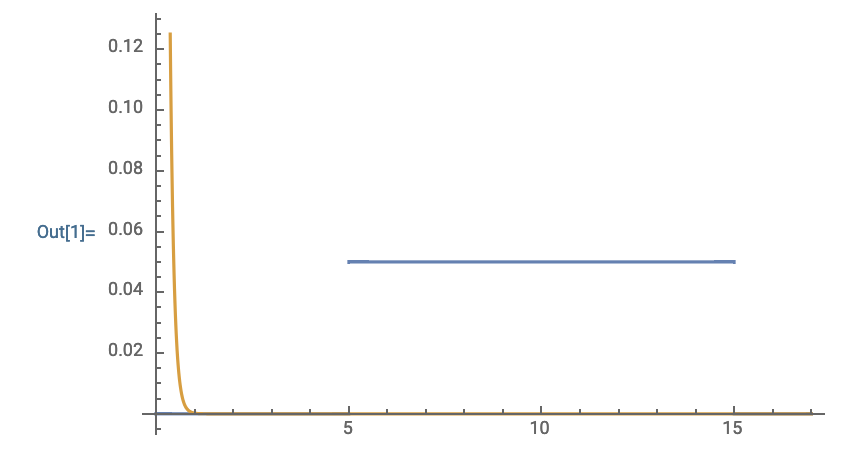
\includegraphics[scale=0.5]{graph1.png}

\item Compute the Bayes error rate for this problem within 3 decimal places of accuracy

The Bayes error rate for this problem is 
\begin{multline}
	\int_0^5 P(c_2|x)p(x) dx + \int_5^{15} P(c_1|x)p(x) dx + \int_{15}^\infty P(c_2|x)p(x)dx = \\
	0 + \int_5^{15} 10e^{-10x}*0.5 + 0 = \frac{e^{100}-1}{2e^{150}} = 9.644*10^{-23}
\end{multline}

\item Answer parts 1, 2, and 3 above but now with $p(c_1) = 0.4$ and $p(c_2) = 0.6$.

The decision boundries are unchanged, the new sketch is 

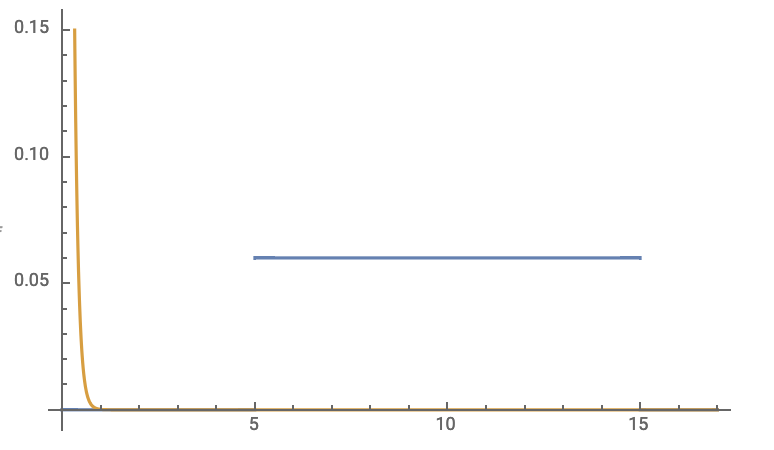
\includegraphics[scale=0.5]{graph2.png}

and the new error rate is 
\begin{equation}
	\int_5^{15} 10e^{-10x}*0.4 = \frac{2e^{100}-2}{5e^{150}} = 7.715*10^{-23}
\end{equation}

\end{enumerate}
    
\subsection*{Problem \ref:  Optimal Decision Regions and Bayes Error  for One-Dimensional Gaussians}

Consider a classification problem with 2 classes $c_1$ and $c_2$ and a single real-valued feature vector $X$, where class 1 has a Gaussian density $p(x|c_1)$ with parameters $\mu_1$ and $\sigma_1^2$, and class 2 has a Gaussian density $p(x|c_2)$ with parameters $\mu_2$ and $\sigma_2^2$.  
\begin{enumerate}
\item Derive equations that define the locations of the optimal decision regions as a function of the parameters.

The optimal decision regions are where $p(x|c_1)p(c_1) = p(x|c_2)p(c_2)$, which for these distributions is equal to 
\begin{equation}
	\frac{p(c_1)}{\sqrt{2\pi\sigma_1^2}}e^{-\frac{(x-\mu_1)^2}{2\sigma_1^2}} = 
	\frac{p(c_2)}{\sqrt{2\pi\sigma_2^2}}e^{-\frac{(x-\mu_2)^2}{2\sigma_2^2}}
\end{equation}

\item Now assume $\mu_1 = 0$ and $\sigma_1^2 = 1$ and $\mu_2=3$ and $\sigma_2^2 = 3$. Also assume $p(c_1) = p(c_2) = 0.5$.  Draw or plot each of $p(x|c_1)p(c_1)$ and $p(x|c_2)p(c_2)$, as a function of $x$, on the same plot, clearly showing the optimal decision boundary (or boundaries).

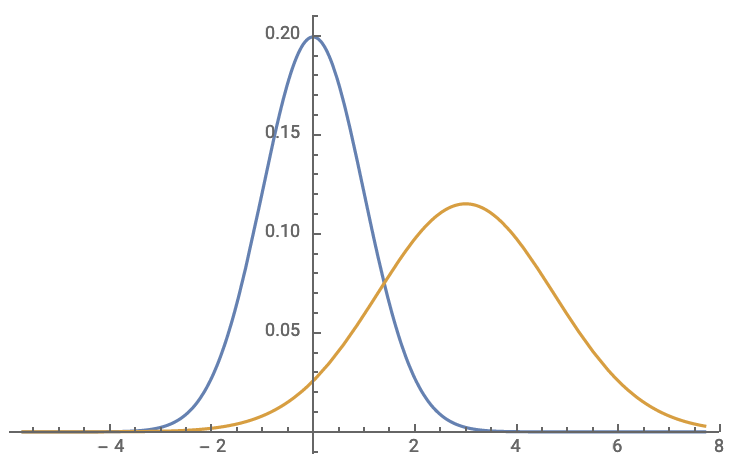
\includegraphics[scale=0.5]{graph3.png} \\
The decision boundries are at the points where the two curves intersect, which are roughly $x=1.398$ and $x=-4.398$.

\item Estimate the Bayes error rate for this problem within 3 decimal places of accuracy (you will need to use numerical tables or call a numerical approximation function for evaluating integrals of the Gaussian density function).

For these boundries, the Bayes error is equal to
\begin{equation}
	\int_{-\infty}^{-4.398} P(c_1|x)p(x) dx + \int_{-4.398}^{1.398} P(c_2|x)p(x) dx + \int_{1.398}^\infty P(c_1|x)p(x)dx
\end{equation}
Using integral estimation software on the PDF's of these gaussians, these integrals are equal to around $2.73132*10^{-6}+0.0887477+0.0405283 \approx 0.129$

\end{enumerate} 

 
 
\subsection*{Problem \ref: Decision Regions for Gaussian Multivariate Models}

Consider a 2-class classification problem with $d$-dimensional real-valued inputs $\ux$, where the class-conditional densities, $p(\ux|c_1)$ and $p(\ux|c_2)$ are multivariate Gaussian with different means $\umu_1$ and $\umu_2$ and a common covariance matrix $\Sigma$, with class probabilities $P(c_1)$ and $P(c_2)$.
\begin{enumerate}
\item Write the discriminant functions for this problem in the form of
$g_1(\ux) = \log p(x|c_1) + \log p(c_1)$ (same for $g_2(\ux)$).

The log of the PDF of the multivariate normal distribution is 
\begin{equation}
	-\frac{d}{2}log(2\pi)-\frac{1}{2}log(det(\Sigma))-\frac{1}{2}(x - \mu)^T\Sigma^{-1}(x-\mu)
\end{equation}
Therefore
\begin{equation}
	g_i = -\frac{d}{2}log(2\pi)-\frac{1}{2}log(det(\Sigma))-\frac{1}{2}(x - \mu_i)^T\Sigma^{-1}(x-\mu_i) + log(P(c_i))
\end{equation}
with $i=(1,2)$.

\item Prove that the optimal decision boundary, at $g(\ux) = g_1(\ux) - g_2(\ux) = 0$, can be written in the form of a linear discriminant, $\uw^t \ux + w_0 = 0$, where $\uw$ is a $d$-dimensional weight vector and $w_0$ is a scalar, and clearly indicate what $\uw$ and $w_0$ are in terms of the parameters of the classification model.

$g_1 = g_2$ is equivalent to 
\begin{equation}
	\frac{1}{2}(x - \mu_1)^T\Sigma^{-1}(x-\mu_1) + log(P(c_1)) = 
	\frac{1}{2}(x - \mu_2)^T\Sigma^{-1}(x-\mu_2) + log(P(c_2))
\end{equation}
Since 
\begin{equation}
	(x-\mu)^T\Sigma^{-1}(x-\mu_i) = x^T\Sigma^{-1}x - 2(\Sigma^{-1}\mu)^Tx+\mu^T\Sigma^{-1}\mu
\end{equation}
our decision boundary reduces to where
\begin{equation}
	(\Sigma^{-1}\mu_1)^Tx+\mu_1^T\Sigma^{-1}\mu_1 + log(P(c_1)) = 
	(\Sigma^{-1}\mu_2)^Tx+\mu_2^T\Sigma^{-1}\mu_2 + log(P(c_2))
\end{equation}
or 
\begin{equation}
	(\Sigma^{-1}(\mu_1-\mu_2))^Tx + (\mu_1-\mu_2)^T\Sigma^{-1}(\mu_1-\mu_2) + log(\frac{P(c_1)}{P(c_2)}) = 0
\end{equation}
This is a linear discriminant with $w = \Sigma^{-1}(\mu_1-\mu_2)$ and $w_0 = (\mu_1-\mu_2)^T\Sigma^{-1}(\mu_1-\mu_2) + log(\frac{P(c_1)}{P(c_2)})$.

\item Show that if $P(c_1) = P(c_2)$ then the classifier can be viewed as a ``nearest mean" type of classifier, where a vector $\ux$ is assigned to the mean that it is closest to, and where distance is measured using Mahalanobis distance.

If $P(c_1) = P(c_2)$, all terms of $g_i(x)$ are constant across $i=(1,2)$ except for $-\frac{1}{2}(x - \mu_i)^T\Sigma^{-1}(x-\mu_i)$, which is the square of the Mahalanobis Distance between $x$ and $\mu_i$. 
Thus, the decision will be made entirely upon which value of $i$ gives a lower value for the Mahalanobis distance between $x$ and $\mu_i$, or in other words, which mean $x$ is closest to.

\end{enumerate}
 


\end{document}

\subsection*{Problem \ref: Probabilities from 0/1 Training Data} 
Consider training a model $f(\ux; \ut)$, such as a logistic regression model, with parameters $\ut$. We have
labeled training data $D = \{ (\ux_i, y_i) \}, 1 \le i \le N$, where $y_i \in \{0,1\}$ are class labels.

Consider two different empirical risk functions:
\[
R^{\mbox{emp}}_{\mbox{log}} \ = \ - \frac{1}{N} \sum_{i=1}^N 
y_i \log f(\ux_i ; \ut) + (1 - y_i)  \log (1 - f(\ux_i; \ut) )
\]
and
\[
R^{\mbox{emp}}_{\mbox{mse}} \ = \ \frac{1}{N} \sum_{i=1}^N 
\biggl( y_i - f(\ux_i ; \ut) \biggr)^2
\]

\begin{enumerate}
\item Prove that as $N \to \infty$, that the optimal solution to minimizing 
$R^{\mbox{emp}}_{\mbox{log}} $ is to set $f(\ux ; \ut) = p( y= 1 | \ux, \ut)$ for all values of $\ux$.
\item Prove that as $N \to \infty$, that the optimal solution to minimizing 
$R^{\mbox{emp}}_{\mbox{mse}}$ is to set $f(\ux ; \ut) = E_{p(y | \ux, \ut)}[y]$ for all values of $\ux$, and that $E_{p(y | \ux, \ut)}[y] =  p( y= 1 | \ux, \ut)$ when $y\in \{0,1\}$.
\end{enumerate}
What you have shown in this problem is that for any model $f(\ux ; \theta) $, if it is trained with either log-loss or squared error, the minimum of the loss function occurs when $f(\ux_i ; \ut)  = p( y= 1 | \ux, \ut)$, i.e., model will try to approximate posterior class probabilities $p( y= 1 | \ux, \ut)$. Note that this happens for any model $f$ (including logistic regression and neural networks)  even though the models are only provided with 0's and 1's as target values to train on (i.e., they do not see probabilities during training).